\section{Introduction}

\subsection{Motivation}

\begin{itemize}
    \item multiple sensors per robot resulting in multimodal sensor fusion requirements
    \item depth sensors increasingly used in the field and quality of sensors improve dramatically
    \item performance/compute costs of ICP high
    \item other approaches require many compuations as well, parallelization is major concern for improving performance
    \item due to ICP limitations, combining laserscan and depth sensor hard
    \item ICP requires correspondent in the pointclouds and inital pose
    \item global positioning not easily done, because of local maxima and computational cost of for example particle based approaches
\end{itemize}

\subsection{Problem Definition}

\begin{itemize}
    \item rigid and non-rigid registration
    \item registering depth and range data
    \item Kinect fusion
    \item dependent on initial pose
    \item some algorithms for laserscan matching work on 2D laser scans, but not dense 3D scans
    \item other multi-modal registrations
    \item mining environment
    \item prior high resolution laser scans exist
    \item bad lighting conditions
\end{itemize}

\subsection{Other Approach}

\begin{itemize}
    \item Scaramuzza\cite{Scaramuzza2007} presented work on registering a camera to a laserscaner using manually selected features in the laserscan and the image
    \item prior conversion of the laserscan to an image dubbed \Glspl{bearing-angle-image}
    \item converted image shows the local geometric structure exposed to the scan

    \item Lin et.al\cite{Lin2017} applied SURF feature detection on \Glspl{bearing-angle-image}
    \item this allows feature based posed estimation with the classical workflow used in SLAM algorithms
\end{itemize}

\subsection{Improvements}

\begin{itemize}
    \item \Glspl{bearing-angle} is calculated in only one direction and can therefore not be rotation invariant
    \item this work proposes \Glspl{flexion-image} that encodes the local geometry in all directions and is rotation invariant
    \item multiple state-of-the-art keypoint detectors and feature descriptors are compared between \Glspl{flexion-image} and \Glspl{bearing-angle-image} on various datasets taken with Kinect v2 and a full Laserscan
    \item evaluation shows better performance of \Glspl{flexion-image} with regard to keypoint quality and feature description
\end{itemize}

\subsection{Structure of this Thesis}

\section{Related Work}

\subsection{Bearing-Angle and SURF}

\begin{itemize}
    \item scaramuzza calibration of laser scan to camera
    \item conversion of laser-scan to bearing angle image
    \item manual selection of corresponding corner features in bearing angle image and color image
    \item rigid transformation calculation with error minimization

    \item Lin et.al use automatic feature extraction on bearing angle image with SURF
    \item use for pose estimation, inital pose for ICP

    \item both formulations of the bearing angle calculation incorrect
    \item scaramuzzas formulation produces sqrt of negative number
    \item lin seem to forget the sqrt of denominator, proper derivation is done in attachement
\end{itemize}
Erratum for Scaramuzza and Lin

\subsection{Rigid and Non-Rigid Pointcloud Registration}

\begin{itemize}
    \item goal is to find a transformation between two point sets that to map one pointset to the other
    \item process is called registration and used in robotics, medicine and field
    \item 6-DoF transformation is a rigid registration and is equivalent to find the common frame of reference of both point clouds
    \item non-rigid registration includes shearing and scaling but can also imply non-linear transformations
    \item non-rigid is not considered in this thesis, because the goal is to find a pose with the precondition of rigid transformation
\end{itemize}

\subsubsection{Correspondence Based Approaches}
\begin{itemize}
    \item ICP with different formulations
    \item point-to-plane ICP
    \item plane-to-plane ICP
    \item generalized ICP
\end{itemize}

\subsubsection{Otha}
\begin{itemize}
    \item normal distribution transformation
    \item coherent point drift
\end{itemize}

\subsection{Multi-Modal Sensor Registration}

\begin{itemize}
    \item Kinect Fusion\cite{newcombe_ismar2011}
    \item dense visual odometrie\cite{kerl_icra2013}
    \item multi-cue photometric registration\cite{corte_2017}
    \item all are focussed on RGB-D data and do not consider dense laser scans
    \item alignment using normalized mutual information
\end{itemize}

\section{Fundamentals}

This section of the thesis introduces the relevant theory and principles building the foundation of the describes approach.

\subsection{Depth Sensors}

\subsubsection{Structured Light}

\begin{itemize}
    \item Kinectv1
    \item Intel Realsense
    \item project grid structure in the world with infrared light
    \item sense the deformation of the grid lines and calculate the distance of an object from this deformation
\end{itemize}

\subsubsection{Time-of-Flight}

\begin{itemize}
    \item range imaging camera system to measure the distance of world point by measuring the time, light needs to travel to the object and back for every pixel of an image
    \item the light source can be a laser or a LED
    \item the technology is related to LIDAR
    \item these camera systems operate faster than LIDAR but have lower resolution
    \item especially in robotics the kinect v2 is commonly found as time-of-flight sensor
\end{itemize}

\subsubsection{LIDAR}

\begin{itemize}
    \item light detection and ranging
    \item measure the time a laser beam requires travels to an obstacle
    \item reflected light is analyzed, both phase shift and time of travel give information about distance
    \item intensity can be measured by some laser scanners as well
    \item broad spectrum of application in various disciplines
    \item can be full resolution 3D scanning or provide vertically sparse scan lines
    \item in this work dense laser scans are of interest
\end{itemize}

\subsection{Image Formation and Camera Models}

\subsubsection{Pinhole camera model}

Forward projection, backward projection.
Very common, and depth sensor can be modeled with this

\subsubsection{Equirectangular Camera Model}

Image to sphere, forward and backward projection
Laser scan can be modeled with this
Vertical field of view is limited

\subsubsection{Range and Depth Conversion}

There are two possible conventions on how to store depth data.
Depth is the distance from coordinate plane.
Range is the length of the light ray that corresponds to a pixel value.
Depth-Sensors usually provide depth information, LIDAR range information.
For consistency and generality depth data is converted to range data.
This simplifies later conversion and mixing of different camera models.

\subsection{Noise Filtering}

Commonly used a preprocessing step for other algorithms.
Measurements are usually noisy. Filtering evens out the signal
Can be normal like gaussian blur or box filter.
Can be edge preserving to keep edge features.

\subsection{Keypoint Detection and Feature Description}

Technique from computer vision on color images.
Salient regions of the image are of interest to extract further information.
Can be used for triangulation, for example in stereo camera systems.
Can be used to determine trajectory of single camera.
Can be used to recognize a place or search for similar images --- document extraction.

Common features are corners, edges and more complex features that are extracted with the common algorithms described later.
Each feature has a pixel location in the image and optionally a response and a size.

Recognizing such a salient point in the image from another image that is taken from a different perspective or for example after a change in the scene requires to model the local surroundings of that spot.
This step is done by feature descriptors, sometimes called keypoint descriptors.

Such a descriptor builds a model of the region around that specific keypoint.
Such a model can be a histogram of brightness values at various distances around that point.
Optionally either the descriptor or the keypoint can be assigned a rotation.
This step is not consistently done be one or the other and sometimes saved completly, because not rotation is expected to happen and the computational cost can be saved.
The model is then stored as a vector.
This vector can be of type real or contains boolean values, too.
The length varies from algorithm to algorithm, but 64 elements or more are common dimensions.
Descriptors that result in booleans can for example sample the environment of a keypoint in a predefined order and just store if the brightness is higher or lower then the previous sample.

The last and final step is matching descriptors, for simplicity reasons the case of two consecutive images in a video stream is choosen to demonstrate the principle workings.
The simplest method is to calculate the distance of each descriptor of the first image with each descriptor of the second image.
Choosing the right norm is crucial for both accuracy and speed of this step.
Dense real descriptors usually choose the L2 or L1 norm resulting in higher computational cost due to the floating point operations.
Binary descriptors use the Hamming Norm which is very cheap to compute.
Both descriptors are XOR'ed together and the number of set bits of the result is the distance of these descriptors.

Conceptually, descriptors with minimal distance correspond to each other.

Further heuristics should be applied to reduce the number of false positives and to improve the results.
The first heuristic is called cross checking. Descriptors correspond only if the distance of the descriptors is minimal in both directions.
That means that descriptor 1 has no closer descriptor in image 2, and the matched descriptor from image 2 has no closer descriptor in image 1 then descriptor 1.

The second commonly used heuristic is the lowe ratio check\cite{lowe_ijcv2004} that requires that the second best match for a descriptor must succeed a certain distance ratio.

Another simple heuristic is a maximum accepted descriptor distance.
This is different for descriptor type, -size and matching norm and requires empirical data for a given use case.
Therefore, it is not simple to define which value to choose but requires careful consideration of the operational environment and parameters in use.

More complicated preprocessing can be done to reduce the number of descriptors to match.
Some keypoints can be discarded to achieve a good distribution over the image and avoid clusters of keypoints.
Keypoints can be discarded on the response or size.
Filtering by response is commonly done when selecting only e.g. 300 keypoints.
If apriori information of the approximate motion of the camera is known matches can be ranked based on the expected displacement of the keypoint given the known motion.

In information retrieval scenarios, e.g.~a search engine for similar images, further processing is necessary.
This includes clustering of descriptors and only storing a representative as well as dimension reduction and hierarchical data structures to store the descriptors in to make the matching of a vast number of descriptor feasable.

\subsection{Statistics of Binary Classifiers}

To evaluate the performance of keypoint detection and feature matching such a system can be considered a binary classifier.
The clasification task is to determine if a keypoint X1 of image I1 corresponds with keypoint X2 in image I2 with a true or false outcome.

The evaluation of the performance of various keypoint detection and matching algorithms makes extensive use of this idea.
As with most statistics it is necessary to consider the distribution of a quantity and analyze it from multiple view points.
Therefor the final evaluation will consider other criteria, like keypoint distribution and number of keypoints per frame as well.

\begin{itemize}
    \item error categories, true positive, true negative, false postive and false negative
    \item contingency-table
    \item leading to accuracy (percentage of correct decisions)
    \item this leads to various ratios describing the performance 
    \item common measures precision-recall
    \item common measures sensitivity-specificity
    \item comparibility in \gls{ROC} space
    \item informedness of the system as youden index and correspondence to \gls{ROC} space
    \item degress of freedom in roc space and generally dependence on absolute numbers for decision 
\end{itemize}

\section{Depth Image Processing}

As with most sensor data the sensory input requires some preprocessing.
Error sources for depth sensors are absorption or reflexion of the infrared light, for example by water or glass.
Additionally each sensors has a range of sensing.
Every object too near or far can not be measured, sharp edges produce shadows.
Those conditions lead to missing distance values for such pixels, represented by zeros.

Another source of error are inaccurate measurements by the sensor.
Some sensors, like the Intel Realsense even have visible waves in the sensor output.
Additionally, depth images are discretized to integer precision.

These errors can be partially mitigated by preprocessing and filtering.

\subsection{Depth Image Impainting}

Filling holes in the depth image can be done with depth image impainting techniques.

\begin{itemize}
    \item interpolation between neighbouring pixels
    \item using the color image to find edges
    \item estimation of planes or other geometric primitives and filling the depth values to match those primitives
\end{itemize}

Those techniques have different level of quality.
Manual testing for the scenes presented later showed no noticeable improvement.
This is due to the walls inside the mine have many sharp edges that do not follow normal manbuild structures.
Impainting-techniques work better when planes and bigger surfaces can be used to estimate the real world geometry, which is not the case for the experiments.

\subsection{Edge-Preserving Filtering}

Filtering is an operation to reduce the impact of sensor noise.
One common filter is gaussian blur or the computationally cheaper box filter.
Those filters distribute each sensory value over a local neighbourhood with different weights.
This reduces white noise but blurs edges and shapes as well.
Therefore, these filters are not edge preserving and undesirable for the use-case of this work.
As described later, preserving sharp edges is requirement to be able to extract features from the converted depth images.
Using proven implementations from OpenCV\cite{opencv_library}.

\subsubsection{Median Blur}

\begin{itemize}
    \item kernel of odd size greater then one $ksize \times ksize$
    \item replacing the center pixel with median over all pixel in that kernel
    \item computationally cheap, easy to utilize SIMD instructions
    \item edge preserving and smoothing
    \item filling single pixel errors with reasonable value of surrounding
    \item cite a paper/book
\end{itemize}

\subsubsection{Bilateral Filter}

\begin{itemize}
    \item edge preserving filter that considers both spatial proximity as well as proximity of surrounding values
    \item smooths out smaller fluctuations in local neighbourhood, but maintains sharp edges
    \item cite proper paper
\end{itemize}

\subsection{Conversion from Depth-Image to Feature Image}

For transition from depth-based to feature-based registration a prior conversion from depth values to a derived image is required.
Every feature-image is calculated on range data in floating point format.
Conversion from integer data does no further processing then simply type conversion.

\subsection{\Glspl{bearing-angle-image}}

\begin{figure}[H]
    \centering
    \tikzset{every picture/.style={line width=0.75pt}} %set default line width to 0.75pt        

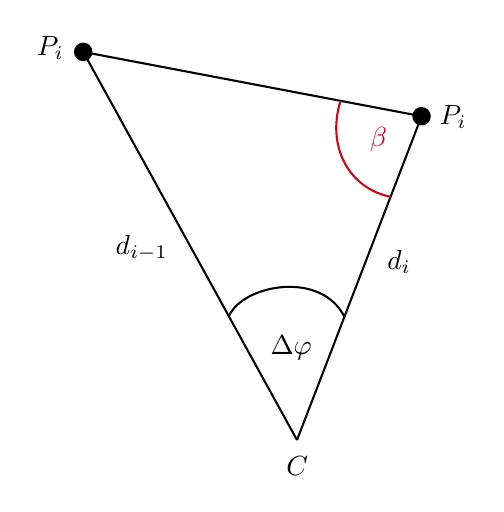
\begin{tikzpicture}[x=0.75pt,y=0.75pt,yscale=-1,xscale=1]
%uncomment if require: \path (0,227.75); %set diagram left start at 0, and has height of 227.75

%Straight Lines [id:da05017383740499093] 
\draw    (38.83,15.67) -- (141.83,202.67) ;


%Straight Lines [id:da6895513561877372] 
\draw    (201.83,46.67) -- (141.83,202.67) ;


%Curve Lines [id:da10253757735662583] 
\draw [color={rgb, 255:red, 0; green, 0; blue, 0 }  ,draw opacity=1 ]   (109,143) .. controls (115.83,127.67) and (153.83,120.67) .. (164.83,143.67) ;


%Straight Lines [id:da3851492122035306] 
\draw    (38.83,15.67) -- (201.83,46.67) ;


%Curve Lines [id:da7052636563383052] 
\draw [color={rgb, 255:red, 208; green, 2; blue, 27 }  ,draw opacity=1 ]   (162.83,39.17) .. controls (155.83,61.17) and (166.9,81.48) .. (186.9,85.48) ;


%Shape: Circle [id:dp08101382020617043] 
\draw  [fill={rgb, 255:red, 0; green, 0; blue, 0 }  ,fill opacity=1 ] (197.88,46.67) .. controls (197.88,44.49) and (199.65,42.72) .. (201.83,42.72) .. controls (204.01,42.72) and (205.78,44.49) .. (205.78,46.67) .. controls (205.78,48.85) and (204.01,50.62) .. (201.83,50.62) .. controls (199.65,50.62) and (197.88,48.85) .. (197.88,46.67) -- cycle ;
%Shape: Circle [id:dp7397482298206297] 
\draw  [fill={rgb, 255:red, 0; green, 0; blue, 0 }  ,fill opacity=1 ] (34.88,15.67) .. controls (34.88,13.49) and (36.65,11.72) .. (38.83,11.72) .. controls (41.01,11.72) and (42.78,13.49) .. (42.78,15.67) .. controls (42.78,17.85) and (41.01,19.62) .. (38.83,19.62) .. controls (36.65,19.62) and (34.88,17.85) .. (34.88,15.67) -- cycle ;


% Text Node
\draw (139,158) node [color={rgb, 255:red, 0; green, 0; blue, 0 }  ,opacity=1 ] [align=left] {$\displaystyle \Delta $$\displaystyle \varphi $};
% Text Node
\draw (181,58) node [color={rgb, 255:red, 208; green, 2; blue, 27 }  ,opacity=1 ] [align=left] {$\displaystyle \beta $};
% Text Node
\draw (191,117) node  [align=left] {$\displaystyle d_{i}$};
% Text Node
\draw (67,110) node  [align=left] {$\displaystyle d_{i-1}$};
% Text Node
\draw (217,47) node  [align=left] {$\displaystyle P_{i}$};
% Text Node
\draw (23,14) node  [align=left] {$\displaystyle P_{i}$};
% Text Node
\draw (142,215) node  [align=left] {$\displaystyle C$};


\end{tikzpicture}
%
    \caption[Schematic Representation of Bearing-Angles]{This figure shows the relationship of the light rays that form the \gls{bearing-angle}.}
\end{figure}

Existing literature\cite{Scaramuzza2007,Lin2017} proposes \Glspl{bearing-angle-image} were each pixel is the angle between the current point, the optical center and the previous point.
The neighbourhood relationship can be choosen arbitrarily resulting in four first-order \Glspl{bearing-angle-image}, horizontal, vertical, diagonal and antidiagonal.
The second variable is the direction the angle is calculted, e.g.~for horizontal images it can be calculated from left-to-right or right-to-left.
This does not exhibit new information, because the angle of the other direction is immediatly known from the fact that the sum of the angles is $180\degree$.
Nontheless, the direction must be defined to obtain stable visual features.

The formula for the \gls{bearing-angle} $\beta$ is derived with the cosine theorem.
For the horizontal left-to-right calculation the formula is as follows.
\begin{align}
    \beta&= \arccos%
            \frac{d_{i,j} - d_{i-1,j} \cos \Delta\varphi}%
                 {\sqrt{d_{i,j}^2 + d_{i-1,j}^2 - 2 d_{i,j} d_{i-1,j} \cos \Delta\varphi}}
\end{align}
Using a different direction or other neighbourhood relation the indices for the depth values need to be changed and a different angular resolution needs to be calculated.
The \Gls{bearing-angle} is in the range $(0, \pi)~rad$ and gets scaled accordingly.

\subsection{\Glspl{flexion-image}}\label{flexion-image-section}

Each pixel of a \Gls{flexion-image} is the dot-product of the local normal
calculated from horizontal and vertical neighbouring pixel with the
normal calculated with the diagonal neighbours.
Figure~\ref{fig:flexion-image-scetched} demonstrates the disparity of both normals for an arbitrary surface patch.
The normal calculated from the diagonal and vertical neighbouring vertices are drawn in blue and the normal calculated with the diagonals red.
Both normal-vectors are drawn with their origin in the central depth value.

\begin{figure}[H]
    \centering
    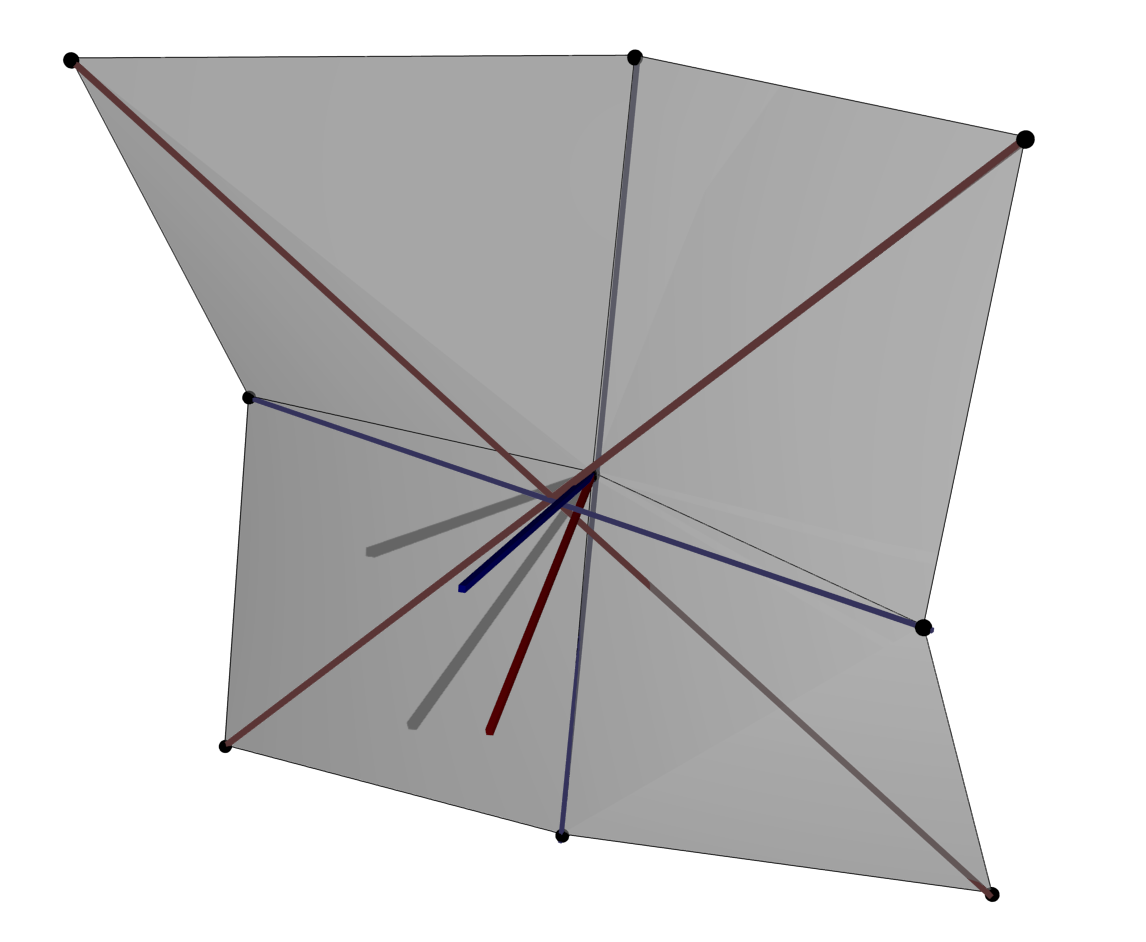
\includegraphics[width=0.6\textwidth]{images/scetch_flexion.png}
    \caption[Schematic Representation of Flexion]{This figure demonstrates how flexed surfaces have different normals for diagonal and non-diagonal estimation. This difference is utilized as measure for flexion.}%
    \label{fig:flexion-image-scetched}
\end{figure}

The flexion $f$ is defined as
\begin{align}
    f &= \abs{n_1 \cdotp n_2}
\end{align}
Because $n_1$ and $n_2$ are of length $1$ the value of $f$ is in the range $[0, 1]$ and gets scaled accordingly.

The smaller the dot-product gets, the higher is the local flexion of the
surface. This local property of the geometry then results in visual
features detectable with classical feature detectors and descriptors like
\Gls{sift} or \Gls{surf}.

\subsubsection{Curvature}

As a different analytical approach to producing feature images the calculation of the \gls{curvature} for each depth value.
The two common measures of curvature in differential geometry are \gls{gaussian-curvature} and \gls{mean-curvature}\cite{Kuhnel2008}.

If the function is known as a graph the \Gls{gaussian-curvature} can be estimated using the derivatives of the function.
For depth data each depth value is a sample of this function graph and numeric approximation of the derivatives allows the calculation of the curvature.
\begin{align}
    \mathfrak{K} &= \frac{f_{uu} f_{vv} - f_{uv}^2}{{(1 + f_u^2 + f_v^2)}^2}
\end{align}
With
\begin{align*}
    f_{x} &= \frac{y_1 - y_0}{\Delta x} \\
    f_{xx} &= \frac{y_1 + y_{-1} - 2 y_0}{{\Delta x}^2}
\end{align*}
as approximation for the derivatives.

Similarly, the \Gls{mean-curvature} can be calculated with a different formula.
\begin{align}
    \mathfrak{H} &= \frac{{(1 + f_{v}^2)} f_{uu} - 2 f_u f_v f_{uv} + {(1 + f_u^2)} f_{vv}}{2 \sqrt{1 + f_u^2 + f_v^2}^3}
\end{align}
Both measures of curvature are $\mathfrak{K},\mathfrak{H} \in {\rm I\!R}$.
To convert them into a meaningful grayscale image they need to be clamped to arbitrary bounds, that can be choosen based on visual distinctiveness or other heuristics.
After clamping the values are scaled and quantized accordingly.

\subsubsection{Multi-Directional Bearing Angle}

The \gls{max-curve-image} tries generalize the \gls{bearing-angle} to be rotation invariant as it takes the \gls{bearing-angle} in each direction into account.
Additionally to the left-sided \gls{bearing-angle} the right-sided angle is calculated as well and finally added.

\begin{figure}
    \tikzset{every picture/.style={line width=0.75pt}} %set default line width to 0.75pt        

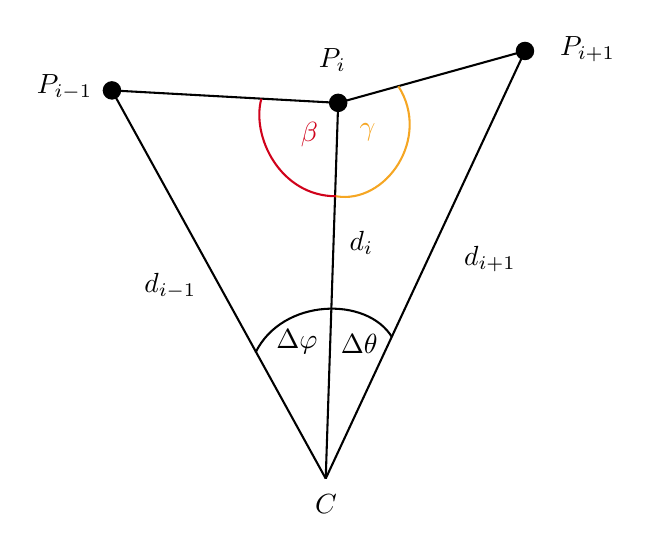
\begin{tikzpicture}[x=0.75pt,y=0.75pt,yscale=-1,xscale=1]
%uncomment if require: \path (0,252.25); %set diagram left start at 0, and has height of 252.25

%Straight Lines [id:da05017383740499093] 
\draw    (46.83,26.67) -- (149.83,213.67) ;


%Straight Lines [id:da6895513561877372] 
\draw    (155.83,32.67) -- (149.83,213.67) ;


%Curve Lines [id:da10253757735662583] 
\draw [color={rgb, 255:red, 0; green, 0; blue, 0 }  ,draw opacity=1 ]   (116,153) .. controls (128.83,126.67) and (169.83,125.67) .. (181.83,145.67) ;


%Straight Lines [id:da3851492122035306] 
\draw    (46.83,26.67) -- (155.83,32.67) ;


%Curve Lines [id:da7052636563383052] 
\draw [color={rgb, 255:red, 208; green, 2; blue, 27 }  ,draw opacity=1 ]   (118.83,30.67) .. controls (113.83,48.67) and (127.83,77.67) .. (154.83,77.67) ;


%Shape: Circle [id:dp08101382020617043] 
\draw  [fill={rgb, 255:red, 0; green, 0; blue, 0 }  ,fill opacity=1 ] (151.88,32.67) .. controls (151.88,30.49) and (153.65,28.72) .. (155.83,28.72) .. controls (158.01,28.72) and (159.78,30.49) .. (159.78,32.67) .. controls (159.78,34.85) and (158.01,36.62) .. (155.83,36.62) .. controls (153.65,36.62) and (151.88,34.85) .. (151.88,32.67) -- cycle ;
%Shape: Circle [id:dp7397482298206297] 
\draw  [fill={rgb, 255:red, 0; green, 0; blue, 0 }  ,fill opacity=1 ] (42.88,26.67) .. controls (42.88,24.49) and (44.65,22.72) .. (46.83,22.72) .. controls (49.01,22.72) and (50.78,24.49) .. (50.78,26.67) .. controls (50.78,28.85) and (49.01,30.62) .. (46.83,30.62) .. controls (44.65,30.62) and (42.88,28.85) .. (42.88,26.67) -- cycle ;
%Shape: Circle [id:dp7936487176657823] 
\draw  [fill={rgb, 255:red, 0; green, 0; blue, 0 }  ,fill opacity=1 ] (241.88,7.67) .. controls (241.88,5.49) and (243.65,3.72) .. (245.83,3.72) .. controls (248.01,3.72) and (249.78,5.49) .. (249.78,7.67) .. controls (249.78,9.85) and (248.01,11.62) .. (245.83,11.62) .. controls (243.65,11.62) and (241.88,9.85) .. (241.88,7.67) -- cycle ;
%Straight Lines [id:da7225304487809803] 
\draw    (245.83,7.67) -- (149.83,213.67) ;


%Straight Lines [id:da15289701870660388] 
\draw    (155.83,32.67) -- (245.83,7.67) ;


%Curve Lines [id:da9153553751002029] 
\draw [color={rgb, 255:red, 245; green, 166; blue, 35 }  ,draw opacity=1 ]   (154.83,77.67) .. controls (178.83,81.67) and (200.83,49.67) .. (184.83,24.67) ;



% Text Node
\draw (136,148) node [color={rgb, 255:red, 0; green, 0; blue, 0 }  ,opacity=1 ] [align=left] {$\displaystyle \Delta $$\displaystyle \varphi $};
% Text Node
\draw (142,48) node [color={rgb, 255:red, 208; green, 2; blue, 27 }  ,opacity=1 ] [align=left] {$\displaystyle \beta $};
% Text Node
\draw (167,100) node  [align=left] {$\displaystyle d_{i}$};
% Text Node
\draw (75,121) node  [align=left] {$\displaystyle d_{i-1}$};
% Text Node
\draw (153,12) node  [align=left] {$\displaystyle P_{i}$};
% Text Node
\draw (24,25) node  [align=left] {$\displaystyle P_{i-1}$};
% Text Node
\draw (150,226) node  [align=left] {$\displaystyle C$};
% Text Node
\draw (276,7) node  [align=left] {$\displaystyle P_{i+1}$};
% Text Node
\draw (229,108) node  [align=left] {$\displaystyle d_{i+1}$};
% Text Node
\draw (170,47) node  [align=left] {$\displaystyle \textcolor[rgb]{0.96,0.65,0.14}{\gamma }$};
% Text Node
\draw (166,149) node [color={rgb, 255:red, 0; green, 0; blue, 0 }  ,opacity=1 ] [align=left] {$\displaystyle \Delta $$\displaystyle \theta $};


\end{tikzpicture}

    \caption[Schematic Representation of the Max-Curve]{The Max-Curve composes two \Glspl{bearing-angle} in vertical, horizontal, diagonal and antidiagonal direction. The maximum angle is then selected as pixel value.}
\end{figure}

This makes the measure more robust to rotation, but does not produce good features.
\begin{align}
    B &= \max{\{B_{diagonal}, B_{antidiagonal}, B_{horizontal}, B_{vertical}\}}
\end{align}

\subsubsection{Viability of Conversions}

\begin{itemize}
    \item effect of noisy input
    \item soundness and mathematical foundation
    \item computational complexity
    \item Discussion of characteristic for Bearing Flexion.
\end{itemize}

\subsubsection{Implementation Notes}

Formulas pictures and short computational evaluation.
Each implementation is independent of the camera model.
Describe the concepts required for implementation.
Both serial and parallel execution.
Parallel execution is done row-wise over all cores using CppTaskflow based Task Scheduling.
No explicit use SIMD, because OpenCV\cite{opencv_library} is used for data storing proper memory alignment is already ensured.
Specialized optimiziation should allow the use of SIMD with OpenCV's Hardware Abstraction Layer.

Focus on correctness and generality.
Provided implementation should rather serve as reference implementation that can be used to validate optimized implementations.

\begin{lstlisting}
template <template <typename> typename Intrinsic,
          typename Real>
inline constexpr bool is_intrinsic_v =
  std::is_floating_point_v<Real>
  &&
  std::is_same_v<typename Intrinsic<Real>::real_type, Real>
  &&
  std::is_invocable_r_v<
    int,
    decltype(&Intrinsic<Real>::w),
    Intrinsic<Real>
  >
  &&
  std::is_invocable_r_v<
    int,
    decltype(&Intrinsic<Real>::h),
    Intrinsic<Real>
  >
  &&
  std::is_invocable_r_v<
    math::sphere_coord<Real>,
    decltype(&Intrinsic<Real>::template pixel_to_sphere<int>),
    Intrinsic<Real>,
    math::pixel_coord<int>
  >
  &&
  std::is_invocable_r_v<
    math::sphere_coord<Real>,
    decltype(&Intrinsic<Real>::template pixel_to_sphere<Real>),
    Intrinsic<Real>,
    math::pixel_coord<Real>
  >
  &&
  std::is_invocable_r_v<
    math::pixel_coord<Real>,
    decltype(&Intrinsic<Real>::template camera_to_pixel<Real>),
    Intrinsic<Real>,
    math::camera_coord<Real>
  >
  &&
  std::is_invocable_r_v<
    math::pixel_coord<int>,
    decltype(&Intrinsic<Real>::template camera_to_pixel<int>),
    Intrinsic<Real>,
    math::camera_coord<Real>
  >;
\end{lstlisting}

\subsection{Feature Detection and Description}

Introduction to feature detection and matching.
Goals and basic principles.
Use cases like RANSAC, Bag-of-Words and stuff.

\subsubsection{Feature Description and Matching}

maybe delete?

\subsubsection{Filtering Keypoints}

Because feature detection algorithms usually produce hundreds of keypoints per HD image it is necessary to reduce the number and only choose the best keypoints.
Most common way is to filter by response and choose only the best responses.

Segmenting the image in multiple regions and keep a constant number of keypoints per region.
This increase the coverage of the image.
If transformation between two images is calculated it reduces the error from one sided focus and helps to keep track of the image when the camera moves in arbitrary direction.

Filtering by keypoint size is an option. The experiments showed showed many very small keypoints that resulted from noisy sections.
Removing these keypoints improves matching quality and chance for false positives.

\subsubsection{SIFT}

Describe approach of SIFT keypoints and descriptor.

\subsubsection{SURF}

Describe approach of SURF keypoints and descriptor.

\subsubsection{ORB}

Describe combination of ORB algorithms, Harris Corner, FAST features.
BRIEF descriptor on multiple levels.

\subsubsection{AKAZE}

Describe AKAZE and its variants.

\subsubsection{BRISK}

Describe BRISK and AGAST keypoint detector.

\section{Experiments}

Experiments show the feature performance of the converted feature images with various state-of-the-art algorithms.
The provided data ranges from a synthetic scene, images taken by the kinectv2 and one high resolution LIDAR dataset.

Each dataset is processed with different filters and detection algorithm configurations.
Both the pinhole camera model and equirectangular model are used.

\subsection{Datasets}
\subsubsection{Synthetic Scene}

Manually created synthetic scene with geometric primitives.
This shows the effect of translation and rotation on the provided feature images.
Furthermore, it is the basis to judge the feasability of the different feature images.

\subsubsection{Lehrpfad Kinect}

Kinectv2-data from a robot drive in the Reiche Zeche.
It provides groundthruth data from a prior reconstruction after global optimization.
It contains a loop closure and different section of the mining environment, from man made concrete walls to raw stone walls.
The groundthruth poses do not match the scale of the depth sensor anymore, as global optimization adjusted the translation too much.
The rotation is proper, each pose is adjusted with ICP that uses the provided pose as initial guess.

\subsubsection{Office Kinect}



\subsubsection{Laserscans of Reiche Zeche - Wilhelm Stehender Süd}

LIDAR based high resolution scans that are used in the context of mine surveying.
Those scans are not made for robotic or computer vision purposes.
This is the reason, why they have little overlap between each scan.
Special reflectors are used as landmarks to register the point clouds to each other.
Only a subset of the scans is used in this evaluation, to demonstrate the functionality and generality of the approach.
Statistics of the distribution and response of the keypoints are provided.

\subsubsection{LIDAR and Pinhole Camera matching}

One advantage of the feature based approach is mixing highly different depth sensors with ease.
Examplaric scene with data from Kinectv2 sensor and the LIDAR that demonstrates, that matching between those two sensors is possible.
Demonstrate, that prior conversion from equirectangular to pinhole reduces the distortion and therefore change in appearance between different camera models.

% Lehrpfad Ziege ist auch im Wilhelm-Sued-Kinect Datensatz. Damit ist da Equi, +Laserscan Pinhole + Kinect vorhanden

\subsubsection{Synthetic City Scene}

City walkthrough that is used as odometry benchmark.

\subsection{Metrics}

The measure for accuracy for each algorithm is developed in this section.
To determine the performance of the feature-based approach the matching of keypoints is framed in terms of a binary classifier.
For a keypoint correspondence between two images the classification task is to determine if those keypoint correspond to the same point in the real world or not.
This evaluation is done for \Glspl{bearing-angle-image} and \Glspl{flexion-image}.
Only two consecutive images are matched in the pinhole datasets. 
The author does not have knowledge of other approaches to evaluate feature detector and descriptors in this manner.

The following subsections describe each component of this evaluation pipeline in more detail.

\subsubsection{Groundtruth Poses}

The dataset \emph{lehrpfad} provides groundthruth poses from \gls{sfm}.
Due to the global optimization of the \gls{sfm} algorithm these poses do not match with the depth values of the depth images.
Therefore, each pose is refined with an ICP algorithm, namely OpenCV's \emph{FASTICPOdometry} that is based on KinectFusion\cite{newcombe_ismar2011}.

The other pinhole based datasets use only the ICP to provide the groundthrouth pose.
Manual inspection of the results and careful evaluation of the reprojection error validate the correctness of these poses.

\subsubsection{Approach with Backprojection and Distance Threshold}

To measure matching performance, each keypoint of two frames is classified of having a corresponding keypoint in the other frame.
This is done by projecting each keypoints camera coordinates of the previous frame into the current frame using the groundthruth pose.
The new camera coordinates in the current frame are then projected into the image with the intrinsic of the sensor.

This gives two sets of keypoints in the current frame, the keypoints detected in this frame and the keypoints detected in the previous frame, seen from this frames pose.

% TODO: Mathematik dafür einfügen

Corresponding keypoints have a small pixel distance and not corresponding keypoints a bigger pixel distance.
\emph{Small} is a relative value, but the experiments use 2 pixel as threshold.

To classify the result of the descriptor matching each keypoint needs to be analyzed in the following order.
The result are four sets \emph{true-positive}, \emph{false-positive}, \emph{true-negative} and \emph{false-negative}.
The union of these sets are all detected keypoints.

\begin{enumerate}
    \item each matched keypoint correspondence is partitioned into true positive and false positive, using the distance threshold as deciding factor
    \item false negatives are searched in the remaining query-indices, using the same distance threshold
    \item every unhandled keypoint is a \emph{true-negative} as there are no corresponding keypoints left
\end{enumerate}

The partitioning of the keypoints is the foundation for the rest of the evaluation.

\subsubsection{Histograms and Summary Statistics}

To understand the characteristics of a quantity a common approach is to create a histogram.
The histograms counts frequencies for a specific range of data.

Summary statistics are used to reduce a statistical distribution to a few representative values.
Different measures are used, such as the measure of location, distribution and shape.
Those values help to understand and compare different setups and configurations.

Both histograms and its summary statistics are created for the keypoint size, keypoint response, descriptor distance between all keypoints and both descriptor distance for \emph{true-positives} and \emph{false-positives}.

The used measures are
\begin{itemize}
    \item $\min$ and $\max$
    \item median and arithmetic mean
    \item variance and standard deviation
    \item skeweness
\end{itemize}

\subsubsection{Classification Evaluation}

The analysis of the keypoint and descriptor characteristics give already some insight into the algorithm performance but are not suitable for a comparison between different algorithms and do not give insight into potential trade-offs.
For this task the quality of the decisions the keypoint matching algorithm is required.
This is a common task in different scientific disciplines when using the classification formualation from above.
For a broad picture this evaluation uses multiple performance numbers.

\begin{itemize}
    \item precision
    \item recall or sensitivity
    \item fallout or false alarm rate
    \item accuracy or rand-index, as measure of correct decisions of the system
    \item youden-index as measure of informedness of the classifier
\end{itemize}

Each of these single measures gives insight into one aspect of decision making performance.
They do not give a systematic way to judge tradeoffs and no easy way to compare different configurations visually.

For this task, each configuration of an algorithm is plotted in \gls{ROC}-Space as a single point.
These plots make all provided configurations comparable and provide a simple way to judge the performance of a configuration.

\subsection{Parameter Search}

Using the established methods to compare algorithms and configurations the most promising algorithms are tweaked slightly to check, if different parameters show better results.

\subsection{Optimized Parameters}

The optimized parameters are used for another round of evaluation, yielding more results for the following datasets.

\subsection{Odometry on Benchmark Dataset}

Odometrie calculated with best performing algorithms.
Using synthetic dataset blaa.

\section{Results and Discussion}

Show the results for ROC curves.
Present histograms for size, response, distribution and descriptor distances.

\subsection{Algorithm Performance}

Each algorithm with own section, important is distribution, keypoint characteristics, descriptor distances

\subsection{Keypoint-Detector discussion}

\begin{itemize}
    \item Stable Keypoints are important
    \item good Keypoint distribution
\end{itemize}

\subsection{Feature-Descriptor Discussion}

\begin{itemize}
    \item matching performance
    \item Computational Complexity
\end{itemize}

\subsection{Error Discussion}
\begin{itemize}
    \item Sensor noise
    \item Missing Sensordata in combination with noise gives bad flexion images
\end{itemize}

\section{Conclusion}

Very Sensors dependent, Time-of-flight and Laserscan gives the best quality.
SURF does not perform well, Bearing Angle gives lower response and less stability
Flexion is very nice.
FAST based stuff does not perform well, more exotic descriptors neither.
SIFT best, AKAZE very good.
Approach to transform depth image first before processing further works and gives results.

\subsection{Future Work}

\begin{itemize}
    \item BoW
    \item Laserscan with Kinect
    \item Other form of Ransac, that considers the depth information
    \item Performance Optimization, conversion is embarassingly parallel and computed on GPU
\end{itemize}
